%----------------------------------------------------------------------------
\chapter{Bevezetés}

\textbf{Kontextus.} Biometrikus felhasználó azonosítás során a felhasználót saját biológiai jellemzői alapján azonosítjuk. A biometrikus azonosító rendszer a felhasználók biometrikus adatait tárolja és ezek segítségével azonosítja őket. Ezen módszer széleskörű megjelenése a mobiltelefonok fejlődésének köszönhető. Az újabb okostelefonok már képesek ujjlenyomat, arc és hang alapú azonosításra is.
\newline
\newline
A biometrikus azonosításnak számos előnye van a mai hagyományos jelszó alapú bejelentkezéssel szemben. Jelszavakat elveszíthetünk, eltulajdoníthatják tőlünk, illetve ha valaki hozzáfér az email fiókunkhoz már a kétfaktoros jelszavas autentikáció sem biztosít elegendő védelmet~\cite{nicolls_2019}. A biometrikus jellemzők egyedik és fizikailag a felhasználóhoz tartoznak ezért nehéz megszemélyesíteni őket és jóval nagyobb védelmet biztosítanak a jelszavaknál. A nagyobb védelmen kívül gyorsabb és kényelmesebb használni őket, illetve a jelszavakkal ellentétben nem kell emlékezzünk rájuk.
\newline
\newline
\textbf{Probléma.} A jelenleg elterjedt biometrikus azonosítási módszerek körében a biometrikus jel rögzítéséhez bonyolult és drága eszközökre van szükség (retinaszkenner, ujjlenyomat olvasó, digitális tábla aláíráshoz stb.).
\newline
\newline
A biometrikus azonosítási módszerek közül kevésbé elterjedt és jelenleg nagyon kutatott téma a hangalapú felhasználó azonosítás. Ennek előnye, hogy a hang rögzítéséhez nincs szükség drága vagy csak az újabb okostelefonokban található rendszerekre (retinaszkenner, ujjlenyomatolvasó), csupán egy mikrofonra és felhasználói szempontból is kényelmes.
\newline
\newline
Napról napra újabb módszerek, modellek jelennek meg, amelyek nincsenek egységesen rendszerezve, összehasonlítva. Továbbá nem létezik olyan szabad szoftver amellyel tetszőleges modellt használva szimulálhatunk egy beszélőfelismerő rendszert.
\newline
\newline
\textbf{Megvalósítás.} Dolgozatomban bemutatom a beszélőfelismerés fejlődését, megvizsgálom a mai modern neurális hálózat alapú beszélőfelismerő rendszereket, a rendelkezésre álló beszédadatbázisokat. Bemutatok részletesen két beszélőfelismerő modellt, majd meta tanítás alapú optimizációs technikákat. Végül ismertetem az általam implementált android prototípus alkalmazást hangalapú biometrikus azonosításhoz.
\newline
\newline
\textbf{Cél.} A hosszú távú cél egy olyan beszélőfelismerő rendszer létrehozása, amely segítségével összehasonlíthatjuk a különböző modellek teljesítményét, illetve egy általánosan felhasználható beszélőfelismerő alkalmazás létrehozása hangalapú autentikációhoz.
\newline
\newline
\textbf{Kontribúciók.} A dolgozatom a következő kontribúciókat tartalmazza:
\begin{itemize}
	\item Módosított Wavenet architektúra teljesítményének mérése beszélőfelismerésre.
	\item Mérések a voicemap modellen: VoxCeleb adatbázis, triplet loss.
	\item Android prototípus alkalmazás beszélőfelismerésre.
\end{itemize} 


\section{Biometrikus azonosítás}

A biometria az emberek fizikai jellemzőinek mérésével és elemzésével foglalkozik. Alkalmazását tekintve három területet különböztetünk meg~\cite{gemalto_2019}:

\begin{itemize}
	\item Felhasználó ellenőrzés: Az azonosító rendszer a biometrikus adatot egy, korábban rögzített mintához hasonlítja. Ez alapján dönt, hogy a felhasználó hozzáférhet-e a kívánt erőforráshoz. Ilyen egy ujjlenyomat-olvasóval ellátott mobiltelefonon a képernyőzár feloldása. A felhasználó ellenőrzés arra ad választ, hogy az illető az-e akinek mondja magát.
	\item Felhasználó azonosítás: Az azonosító rendszer a biometrikus adatot több korábban vett mintához hasonlítja és arra ad választ, hogy ki a felhasználó; azaz beletartozik-e a korábban eltárolt biometrikus adatokból álló csoportba vagy nem. Ilyen lehet például egy ujjlenyomat-leolvasóval ellátott beléptetőrendszer cégek esetében.
	\item Duplikátum detektálás: Annak ellenőrzése, hogy egy felhasználó egynél többször szerepel-e egy adatbázisban. Csalások, például szociális támogatást többször igénylők kiszűrésére használják.
\end{itemize}
\ \\
Az első biometrikus azonosítási eljárás az ujjlenyomatvételen alapuló személyiségazonosítás volt, amely a modern kriminalisztika világában terjedt el, de manapság már megtalálható okostelefonokban, biometrikus beléptetőrendszerekben is.
\newline
\newline
A biometrikus azonosítást az ún. biometrikus azonosító rendszer végzi el. A folyamat során a biometrikus azonosító rendszer mintát vesz az azonosítandó egyén egy vagy több előre meghatározott fizikai jellemzőjéről, és ezekről digitális lenyomatokat képez. Az első, regisztrációs fázisban a biometrikus minta lenyomatát a rendszer egy adatbázisban eltárolja, majd később az azonosítás során az aktuális mintát összeveti a korábban rögzítettel és dönt az egyezésről. Ahhoz, hogy az ember egy fizikai jellemzőjét biometrikus adatként használhassuk, a következő elvárásokat támasztjuk vele szemben:

\begin{itemize}
	\item Általánosság: A biometrikus adattal minden egyénnek rendelkeznie kell.
	\item Egyediség: A biometrikus adatnak egyedinek kell lennie a releváns populáción belül.
	\item Állandóság: A biometrikus adat nem, vagy csak keveset változzon az idő eltetével.
	\item Mérhetőség: Az biometrikus adat az egyén részéről legyen könnyen mérhető testi adottság.
	\item Teljesítmény: A biometrikus azonosító rendszerek teljesítménye: gyorsaság, pontosság, technológia.
	\item Elfogadottság: A releváns populáción belül a mérési eljárás mennyire elfogadott (emberi méltóság megőrzése).
	\item Biztonság: Mennyire nehéz utánozni, hamisítani a biometrikus adatot?
\end{itemize}

A biometrikus adat lehet fiziológiai (DNS, arc, ujjlenyomat, írisz) vagy viselkedési (hang, írás, gesztusok). Mivel ezek az adatok statisztikai jellegűek, megbízhatóságuk változó. Minél több adat van egy mintában, annál egyedibb, és minél nagyobb a releváns populáció (eltárolt minták összessége), annál valószínűbb, hogy találunk két hasonló mintát. Ennek elkerülésére manapság terjednek a multimódusú biometrikus azonosító rendszerek, amelyek több biometrikus adatot felhasználva végzik ez az ellenőrzés, azonosítás és duplikátum detektálás feladatát. 

\section{Biometrikus rendszerek teljesítménye}

A beszélőfelismerő rendszerek teljesítményének mérésekor a fel nem ismert beszélőket és a rosszul felismert beszélőket vesszük figyelembe. Míg az előbbi kisebb probléma, hiszen a felhasználó újra próbálkozhat, egy illetéktelen felhasználó téves azonosítása jelentős biztonsági rés, ezért minimalizálnunk kell azt.
\newline
\newline
Egy beszélőfelismerő rendszernek kétfajta feladatot adhatunk~\cite{van_leeuwen_2007}:
\begin{itemize}
	\item célzott próba: Két hangmintát adunk a rendszernek egyazon beszélőtől.
	\item nem célzott próba: Két hangmintát adunk a rendszernek két különböző beszélőtől.
\end{itemize} 
\ \\
Mindkét esetben a rendszernek a feladata eldönteni, hogy a két hangminta ugyanattól a felhasználótól származik-e, vagyis megkülönböztetni a célzott és nem célzott próbákat egymástól.
A felismerő rendszer mindkét próba esetén tévedhet, ez két féle hibát von maga után:

\begin{itemize}
	\item hamis pozitív vagy téves riasztás: Egy nem célzott próbát célzottnak tekint.
	\item hamis negatív vagy téves visszautasítás: Egy célzott próbát nem célzottnak tekint.
\end{itemize} 
\ \\
A teljesítmény mérése több módszer is létezik. A NIST a \emph{Detection Cost Function ($C_{det})$} metrikát ajánlja, de ez alkalmazásfüggő. Ebben a fejezetben az EER mérőszámot mutatom be, mert kiszámolása jóval egyszerűbb és nem tartalmaz alkalamazásfüggő paramétereket.

\subsection{Equal Error Rate}
\ \\
Az \emph{Equal Error Rate (EER)} vagy \emph{Crossover Rate (CER)} a biometrikus rendszerek teljesítményének mérésére használatos mérőszám. Az \emph{EER} segítségével tudjuk eldönteni ellenőrzés vagy azonosítás esetén a döntési küszöbérték szintjét, amely mellett a rendszer legjobban teljesít, azaz így optimizáljuk azt. Például beszélőfelismerés esetén két hang különbségét valamekkora távolsággal jellemezzük. Ebben az esetben a küszöbérték alatt azt a távolságot értjük amely szintje alatt a két beszélőt azonosnak, fölötte különbözőnek tekintjük.
\newline
\newline
A biometrikus rendszereket három fontos mérőszámmal jellemezzük. Az FAR, az FRR és az előző kettőn alapuló EER. Az első kettőre általában angolul, a következőképpen hivatkozunk:
\begin{itemize}
	\item False Acceptance Rate (FAR): A tévesen elfogadás esetén a biometrikus rendszer beenged egy illetéktelen felhasználót, azaz hiba miatt mással azonosítja őt. A téves elfogadási ráta ennek a mértéke, a téves elfogadások számának aránya az összes elfogadáshoz képest.
	$$FAR = \frac{FA}{AA},$$
	ahol \emph{FA} a téves elfogadások száma, \emph{AA} pedig az összes elfogadás száma.
	\item False Rejection Rate (FRR): A téves visszautasítás azt jelenti, hogy az illetékes felhasználót a rendszer hiba miatt nem tudja azonosítani. A téves visszautasítási ráta a téves visszautasítások számának aránya az összes visszautasításhoz képest.
	$$FRR = \frac{FA}{AA},$$
	ahol \emph{FR} a téves visszautasítások száma, \emph{AR} pedig az összes visszautasítás száma.
\end{itemize}
Az EER az a pont, ahol az FAR értéke megegyezik az FRR-el.
\newline
\newline
A biometrikus rendszerek karakterisztikáját a \ref{fig:eer} ábra szemlélteti. Vegyük egy beszélőfelismerő rendszer példáját. Látható, hogy a döntési küszöb növelése (mekkora távolság esetén tekintjük azonosnak a két beszélőt) esetén az \emph{FAR} nő és az \emph{FRR} csökken. Ez normális, mert ilyenkor megengedőbbek vagyunk, nagyobb távolság esetén is azonosnak tekintjük a két beszélőt, így több olyan eset lesz amikor két hangminta különböző beszélőktől származik, a rendszer mégis azonosnak tekinti őket és kevesebb olyan amikor két hangminta azonos beszélőtől van és a rendszer mégis visszautasítja. 
\newline
\newline
Ha a küszöböt csökkentjük szigorúbb lesz a rendszer, sokkal kevesebb téves elfogadás lesz, de a szigorúság miatt megnő a téves viszautasítások száma.
\newline
\newline
Az EER a két grafikon metszéspontjában található, ahol FAR és FRR értéke minimális és optimális (az optimizálás alatt érthetjük a kettő szorzatát). Az EER a vízszintes tengelyen megadja az optimális küszöbértéket, a függőlegesen pedig egy hiba rátát. Ez az FRR és FAR hiba rátája, mivel a kettő ebben a pontban megegyezik.

\begin{figure}[!ht]
	\centering
	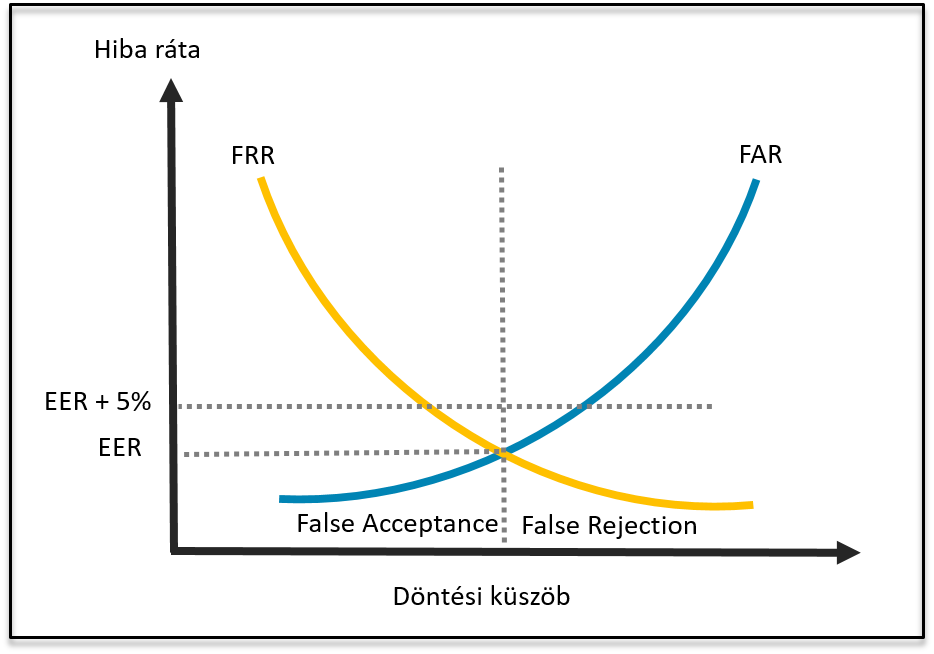
\includegraphics[width=150mm, keepaspectratio]{figures/eer.png}
	\caption{Biometrikus rendszerek karakterisztikája.}
	\label{fig:eer}
\end{figure}
\ \\
Az EER minimalizálásával tehát maximalizáljuk a biometrikus rendszer teljesítményét abból a szempontból, hogy a lehetséges hibák száma így a legkevesebb.
\newpage
\section{Beszélőfelismerés}

Az emberi kommunikáció során fontos feladat a beszélő partner felismerése. A telekommunikációs technológia fejlődése miatt elterjedt a telefonon vagy interneten történő hangalapú kommunikáció; a telefonos felhasználófelismerés mint biometrikus azonosítási módszer megjelent már banki alkalmazásokban, call centerekben és az elektronikus kereskedelemben is (mobiltelefonos vásárlás). Az elektronikus kommunikáció során sokszor csak a beszélő hangjára hagyatkozhatunk, az alapján ismerhetjük fel az illetőt. A beszélőfelismerést háromféle módon végezhetjük~\cite{taufiq_2015}:

\begin{itemize}
	\item Naiv beszélőfelismerés: Az emberi, naiv beszélőfelismerés során az ismerős hangokat meglepően nagy pontossággal ismerjük fel.
	\item Törvényszéki beszélőfelismerés: A törvényszéki szakértői vizsgálat eredménye.
	\item Automatikus beszélőfelismerés: A beszélőfelismerést számítógépes rendszer végzi.
\end{itemize}

A beszélőfelismerés alatt három szűkebb fogalmat értünk. Ha a folyamat során az ismeretlen beszélőről azt ellenőrizzük, hogy az-e akinek állítja magát beszélő ellenőrzésről van szó. Beszélő szegmentáláskor a hangmintát homogén csoportokra bontjuk a beszélő személye alapján. Végül beszélő azonosításról beszélünk, ha az illető hangját rögzített hangok egy csoportjával vetjük össze és azt szeretnénk eldönteni, hogy melyikhez hasonlít a legjobban. Utóbbi felveti a kérdést, hogy mi történik ha a beszélő nem tagja a csoportnak.
\newline
\newline
Emiatt megkülönböztetjük a nyitott és zárt halmazú beszélőazonosítást. Utóbbi esetén csak olyan beszélőket ismerünk fel, akikről van hangminta az adatbázisban, míg az előbbinél ismeretlen beszélők is megjelenhetnek, így ezt is kezelni kell.
\newline
\newline
A beszélőfelismerés továbbá lehet szövegfüggő és szövegfüggetlen attól függően, hogy a felismerő rendszer egy előre meghatározott mondatot vár, vagy bármilyen hangminta alapján képes elvégezni a felismerést.

\section{Az automatikus beszélőfelismerés története}

Az automatikus beszélőfelismerést egy számítógépes program végzi emberi beavatkozás nélkül. Az első automatikus beszédfelismerő rendszert a Texas Instruments fejlesztetése volt és 1977-ben publikálták~\cite{Shaver2016ABR}. A rendszer szövegfüggő beszélőellenőrzésre volt képes és az évek során a téves elutasítási és elfogadási rátája 1$\%$ alatt maradt. A hetvenes évek óta a beszélőazonosító és ellenőrző rendszerek rengeteget fejlődtek kezdve a vektor kvantálástól a GMM modelleken át a mély neurális hálókig.

\begin{figure}[!ht]
	\centering
	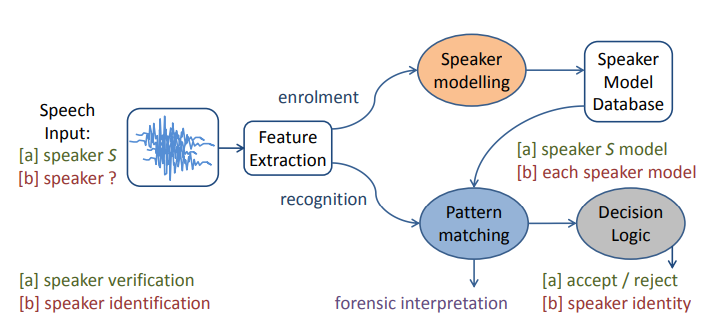
\includegraphics[width=150mm, keepaspectratio]{figures/automatic_speaker_recognition.png}
	\caption{Korábbi automatikus beszélőfelismerő rendszerek architektúrája~\cite{finnian_2014}.}
	\label{fig:automatic_speaker_recognition}
\end{figure}
\ \\
Az automatikus beszélőfelismerő általános működését a \ref{fig:automatic_speaker_recognition} ábra szemlélteti. Működését tekintve két fázist különböztetünk meg: A regisztrációs vagy felvételi fázisban hangmintát veszünk a felhasználótól~\cite{finnian_2014}. Később az azonosítási vagy ellenőrzési fázisban a rendszer újabb mintát kér és az előbbi fázisban eltárolt hangmintával hasonlítja össze. 
\newline
\newline
Mindkét fázis során az első lépés rögzített, alacsonyabb dimenziós \emph{jellemzők kinyerése}, amelynek során a beszédet tömörebb formára hozzuk (pl. hangvektor). Az első, \emph{regisztrációs fázisban} ezután statisztikai modelleket készít az egyes beszélőkhöz a kinyert jellemzők alapján, amelyeket eltárol a beszélő adatbázisban. Ebben a fázisban egy küszöbérték is meghatározásra kerül. \emph{ellenőrzési fázisban} a rendszer kinyeri ugyanazokat a jellemzőket az aktuális hangmintából, majd egy \emph{mintaillesztés} nevű eljárással összehasonlítja a korábban tárolt modellt a jellemzőkkel. Az összehasonlítás eredményét és a küszöbértéket figylembe véve a rendszer dönt az azonosítás vagy ellenőrzés eredményéről.

\begin{enumerate}
	\item beszélő-ellenőrzés esetén megkeresi az ellenőrizendő személyhez tartozó modellt az adatbázisban és összehasonlítja az aktuális jellemzőkkel. Ha az eredmény a küszöbszint felett van, a rendszer egyezést mutat.
	\item beszélőazonosítás esetén az aktuális jellemzőket az összes modellel összehasonlítja, majd a legjobb egyezés mellett dönt. 
\end{enumerate}

\subsection{Jellemző kinyerés}
A jellemző kinyerés célja a dimenzió csökkentése és a beszélőspecifikus információk kinyerése. Mivel a beszéd komplex jel, a beszélő azonosítása szempontjából felesleges információkat is hordoz. Ilyen például a környezet és a csatorna zaja. A kinyert jellemzőket a hangminta terjedelme alapján osztályozzuk. \emph{Rövidtávú jellemzők} a 20-30 ms-os keretekből kinyert mel-frekvenciás és lineáris prediktív kepsztrális együtthatók (MFCC és LPCC)~\cite{taufiq_2015}. A \emph{prozódikus jellemzők} kinyerése 100 ms-os terjedelemben történik és a beszéd ritmusát, a hangmagasságot és a sebességet jellemzik. A hosszútávú jellemzőket a jel akár perc hosszú kereteiből nyerjük ki. Ezek képesek reprezentálni a beszélő akcentusát illetve a szavak szemantikáját és az idiolektust.
\newline
\newline
A beszélőfelismerő rendszerek teljesítményét javította, ha a jellemzőket csak
a hangminta azon részeiből nyerték ki, amikben beszéd is volt. Erre alkalmazott technika a \emph{Voice Activation Detection} (\emph{VAD}).

\subsection{Jellemző normalizálás}

Jellemzőkinyerés során próbáljuk kiszűrni a beszélő szempontjából értékes részéket, ugyanakkor nincs tökéletes jellemző, amely ne változna a környezet hatására. Ezt a változást segítik minimalizálni a normalizálási módszerek.

\subsection{A beszélőfelismerő modellek története}

Kezdetben a vektor kvantálás volt az elterjed modellezési módszer, amit később a \emph{Gaussian Mixture Model} (\emph{GMM}) váltott fel. A GMM egy adathalmazt több normális eloszlás keverékeként ír le és képes nem felügyelt módon klaszterezni az adatokat. Egy beszélőhöz egy valószínűségi sűrűségfüggvényt rendel, amely különböző pontokban kiértékelve (például teszt fázisban a beszélőtől kinyert jellemzők) egy valószínűséget ad a két beszélő hasonlóságára~\cite{taufiq_2015}.
\newline
\newline
A GMM megközelítés főleg beszélőazonosításra alkalmas. Beszélő-ellenőrzéshez szükség volt egy másik modellre is, ami képes leírni minden más beszélőt az ellenőrizendőn kívül. Erre adott megoldást az \emph{Universal Background Model} (\emph{UBM}). Később jobb teljesítményt értek el, ha a teszt fázisban a beszélőkkel először UBM modelleket tanítottak és ezekből származtattak GMM-eket. Ezt nevezik GMM-UBM módszernek.
\newline
\newline
Mivel a tanító és teszt hangminták eltérő hosszúságúak lehetnek, szükség volt egy fix hosszúságú reprezentációra, ezt oldották meg a GMM szupervektorok, amelyeket az akkori megközelítés szerint szupport-vektor gépekkel vagy faktoranalízissel használtak.
\newline
\newline
Az utóbbi két módszer előnyeit kombinálva megszületett az $i-vektorok$, amelyet követve eljutunk a mai state-of-the-art módszerhez, a mély neurális hálózatokhoz (DNN).

\section{Korábbi eredmények}

A \ref{fig:previous_identification_results} ábra korábbi eredményeket mutat szövegfüggetlen beszélőfelismerő rendszerekről. Megfigyelhető, hogy főleg tízes, százas nagyságrendű beszélővel tanított, zárt-halmazú rendszerekről van szó és a tanító mintákat is többnyire laboratóriumi körülmények között rögzítették. Ilyen környezetben könnyebb nagy pontosságot elérni, hiszen nincs háttérzaj, nincsenek új beszélők, a teszt minták nem feltétlenül elég diverzifikáltak. A pontosságot ennek fényében kell értelmezni.

\begin{table}[!ht]
	\resizebox{\textwidth}{!}{%
	\begin{tabular}{*7l} \toprule
		\bfseries Szerző (év)
		& \bfseries Szervezet
		& \bfseries Adatbázis
		& \bfseries Módszer
		& \bfseries Jellemzők
		& \bfseries \begin{tabular}{@{}l@{}} Hang \\ típusa \end{tabular}
		& \bfseries Pontosság \\ \midrule
		
		\begin{tabular}{@{}l@{}} Douglas A. Reynolds  \\  (1995) \end{tabular}
		& \begin{tabular}{@{}l@{}} Lincoln  \\  Laboratory \end{tabular}
		& 49
		& MFCC 
		& \begin{tabular}{@{}l@{}} rövid \\ kifejezések \end{tabular} 
		& telefon 
		& 96.8 \% \\
		
		\begin{tabular}{@{}l@{}} Rabah W.  \\  (2004) \end{tabular}
		& \begin{tabular}{@{}l@{}} King Abdulaziz  \\  University \end{tabular}
		& 20
		& \begin{tabular}{@{}l@{}} SVD-alapú   \\  algoritmus \end{tabular}
		& LPC/Cepstral
		& iroda
		& 94 \% \\
		
		\begin{tabular}{@{}l@{}} Yang Shao  \\  (2008) \end{tabular}
		& \begin{tabular}{@{}l@{}} Ohio State  \\  University \end{tabular}
		& 34 
		& GFCCs 
		& hallási jellemzők
		& telefon
		& \~{}99.33 \% \\
		
		\begin{tabular}{@{}l@{}} P. Krishnamoorthy  \\  (2011) \end{tabular}
		& TIMIT
		& 100 
		& GMM-UBM 
		& MFCC
		& labor
		& 80 \% \\
		
		\begin{tabular}{@{}l@{}} Alfredo Maesa  \\  (2012) \end{tabular}
		& Voxforge.org
		& 250 
		& MFCC 
		& \begin{tabular}{@{}l@{}} spektrális \\ jellemzők \end{tabular} 
		& \begin{tabular}{@{}l@{}} beszéd- \\ adatbázis \end{tabular} 
		& > 96 \% \\

		\begin{tabular}{@{}l@{}} Sharada V. Chougule  \\  (2015) \end{tabular}
		& \begin{tabular}{@{}l@{}} Finolex Academy  \\  of Management \\ and Technology \end{tabular}
		& 97 
		& NDSF 
		& spektrális
		& labor
		& \~{}98-100 \% \\
		
	\bottomrule
	\end{tabular}}
	\centering
	\caption{Korábbi eredmények szövegfüggetlen beszélőazonosítás terén 2017 előtt~\cite{singh_2017}.}
	\label{fig:previous_identification_results}
\end{table}


